\documentclass[../main.tex]{subfiles}
\begin{document}
\chapter{Resumen}
Las ortoferritas de tierras raras \ce{RFeO3} (\ce{R} = catión trivalente de tierra rara), han despertado interés científico gracias a sus propiedades magnéticas como las transiciones de reorientación de espines, switching ultrarrápido a campos bajos y la ferroelectricidad inducida magnéticamente. El interés en el estudio de las ortoferritas, especialmente \neod{} y \sama{}, se debe a su temperatura de reorientación de espín relativamente alta además de sus propiedades dieléctricas \cite{Nakhaei2019} \cite{Sasmal2020}.

En este trabajo se estudian las propiedades morfológicas, estructurales, ópticas, magnéticas y eléctricas del \neod{} y \sama{}, sintetizadas mediante el método sol-gel, con énfasis en su comportamiento magnético y posible multiferroicidad a temperatura ambiente. La síntesis se realizó variando la temperatura de calcinación (600-900\gradoC{} para \neod{} y 700-1000\gradoC{} para \sama) y se realizó un procesado posterior de las muestras mediante la sonicación (0, 2 y 4 h, 292 W).

El análisis termogravimétrico (TGA) reveló que la cristalización ocurre en el rango de 300-500\gradoC{} para ambas ortoferritas.

Las imágenes obtenidas mediante espectroscopía electrónica de barrido (SEM) mostraron partículas porosas que se rompen fácilmente, cuyo tamaño promedio disminuye al aplicar la sonicación ($1.49\pm0.028$ $\mu$m $\shortrightarrow$ $0.98\pm0.023$ $\mu$m para el \neod{} y $2.01\pm0.051$ $\mu$m $\shortrightarrow$ $1.66\pm0.045$ $\mu$m para el \sama{}) y al reducir la temperatura de calcinación, debido a la ruptura de las partículas más grandes, lo cual aumentó significativamente el porcentaje de partículas de diámetro $\geq1$ $\mu$m ($67.29\pm4.0796$\% $\shortrightarrow$ $87.1\pm1.29258$\% para el \neod{} y $55.18\pm2.1034$\% $\shortrightarrow$ $92.62\pm0.91496$\% para el \sama{}).

La espectroscopía de dispersión de energía confirmó la ausencia de contaminantes significativos.

Los patrones obtenidos por difracción de rayos X (DRX) refinados por Rietveld indicaron purezas superiores al 95\% (\neod{} a $\geq$600\gradoC) y 97\% (\sama{} a $\geq$700\gradoC), con trazas de óxidos e hidróxidos.

A través de la espectroscopía UV-Vis se observa que el \textit{band gap} disminuye con la temperatura de calcinación (2.29$\pm$0.004 $\shortrightarrow$ 1.84$\pm$0.003 para el \neod{} y 2.30$\pm$0.001 $\shortrightarrow$ 2.03$\pm$0.002 para el \sama{}), este vuelve a aumentar con el tiempo de sonicación (2.13$\pm$0.009 para el \neod{} y 2.22$\pm$0.002 para el \sama{}).

Las muestras de \neod{} calcinadas a 600\gradoC{} mostraron un comportamiento superparamagnético con una transición de fase magnética a baja temperatura, a diferencia de la muestra calcinada a 900\gradoC{}, la cual presenta un comportamiento ferromagnético débil sin transiciones de fase.

Por otro lado, las muestras de \sama{} presentan una mejoría en sus propiedades ferromagnéticas al ser sometida a sonicación. Muestra un comportamiento complejo a baja temperatura, con múltiples transiciones de fase magnéticas.

Las curvas $P$ vs. $E$ mostraron un comportamiento de histéresis débil a bajos voltajes, con polarizaciones de saturación y remanentes muy bajas independientes de la sonicación ($P_s\approx 0.006$ $\mu$C/cm$^2$ para el \neod{} y $P_s\approx 0.007$ $\mu$C/cm$^2$ para el \sama{}). Este comportamiento desapareció al aumentar el voltaje.
\chapter{Estado del Arte}
\section{Ortoferritas de Tierras Raras}
Los óxidos de tipo perovskita (\ce{ABO3} con A una tierra rara o metal alcalinotérreo y B un metal de transición) son estructuras estudiadas muy comúnmente en el campo de la ciencia de materiales debido a sus propiedades electromagnéticas, ópticas y catalíticas, además de su estabilidad \cite{Wang2019}.

El objeto de estudio de este trabajo son las ortoferritas \ce{RFeO3}, con R una tierra rara, específicamente \ce{R = Nd, Sm}, debido a que presentan un orden magnético intrínseco proveniente de su estructura cristalina, la cual se observa en la figura \ref{fig:estructuras}. 

Esta estructura, con grupo espacial Pbnm, es decir, una celda primitiva ortorrómbica, un plano de deslizamiento tipo b, el cual es perpendicular al eje $\hat{a}$, un plano de deslizamiento tipo n, el cual es perpendicular a $\hat{b}$ y un plano de reflexión perpendicular al eje $\hat{c}$.

La geometría de esta misma estructura favorece también la aparición de momentos dipolares en las celdas cristalinas, lo que hace posible la presencia de ferroelectricidad, haciendo de estas ferritas posibles materiales multiferroicos. \cite{Sharma2024}.
\begin{figure}[H]
    \centering
    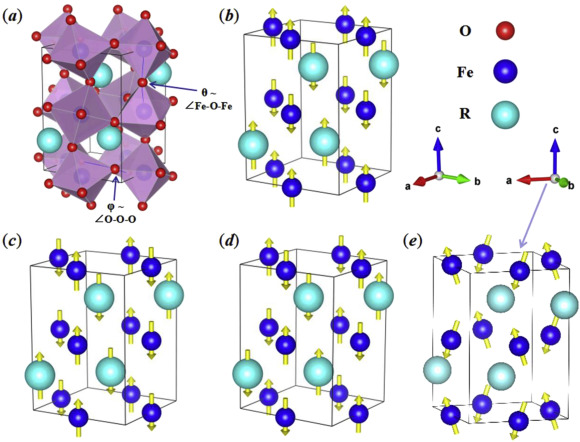
\includegraphics[width=0.5\textwidth]{fig/estructura.jpg}
    \caption{Estructura y posibles alineaciones de las subredes magnéticas de los compuestos \ce{RFeO3}. Tomado de \cite{Wang2019}}
    \label{fig:estructuras}
\end{figure}
Cada una de las estructuras en la figura \ref{fig:estructuras} b-e difieren en el acomodo de sus espines, esto se discutirá a detalle en la sección \ref{sec:magtemp}.


Como se observa en la figura \ref{fig:estructuras} (a), la estructura puede pensarse como una red de octahedros de \ce{FeO6}, superpuesta a una red de átomos de \ce{R}. El ángulo formado por los enlaces \ce{Fe}-\ce{O}-\ce{Fe} es dependiente del radio iónico de \ce{R}, mientras que la temperatura de Néel, la cual se discutirá a detalle en la sección \ref{sec:magtemp}, depende de ambos parámetros, como se muestra en la figura \ref{fig:neelradio}.

\begin{figure}[H]
    \centering
    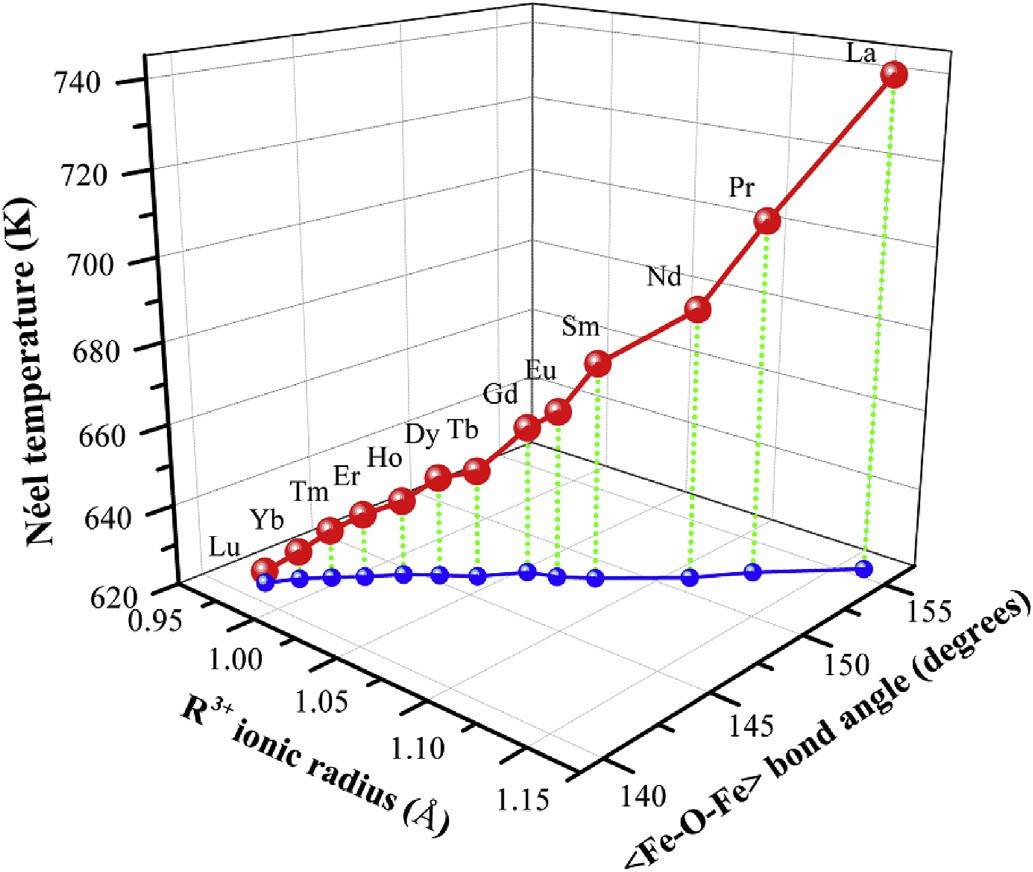
\includegraphics[width=0.5\textwidth]{fig/neelradio.jpg}
    \caption{Temperatura de Néel en función del radio iónico y del ángulo \ce{Fe}-\ce{O}-\ce{Fe}. Tomado de \cite{Wang2019}}
    \label{fig:neelradio}
\end{figure}

\section{Electromagnetismo en Sólidos}
La respuesta de un sólido al aplicar un campo externo, sea éste magnético ($\vec{B}$) o eléctrico ($\vec{E}$), depende de las propiedades intrínsecas del material en cuestión. A pesar de esto, las interacciones a nivel cuántico se manifiestan macroscópicamente como propiedades extensivas, las cuales pueden estudiarse mediante la electrodinámica clásica.

Las ecuaciones de Maxwell pueden modificarse para incluir las contribuciones dependientes de las propiedades del material, considerando que las cargas y corrientes dentro de un éste pueden moverse libremente, o estar ligadas, cada una generando un campo distinto.

$\vec{D}$ y $\vec{H}$ son campos generados por cargas (o corrientes) libres, determinadas por la configuración del sistema, mientras que $\vec{P}$ y $\vec{M}$ son campos generados por cargas (o corrientes) ligadas, determinadas por las propiedades del material \cite{griffiths2023introduction}.

Así, se puede escribir:
\begin{equation}
    \begin{split}
        \vec{D}=\varepsilon_0\vec{E}+\vec{P}\\
        \vec{B}=\mu_0(\vec{H}-\vec{M})
    \end{split}  
    \label{eq:maxwellmacro}
\end{equation}

\subsection{Magnetización en Sólidos}
Esta propiedad depende de las contribuciones de los momentos magnéticos $\vec{m_i}$ de cada electrón dentro del volumen estudiado $V$, es decir:
\begin{equation}
    \vec{M}=\sum_i\dfrac{\vec{m_i}}{V}
    \label{eq:micromag}
\end{equation}
Macroscópicamente, se puede observar que el campo de magnetización depende del campo aplicado $\vec{B}$ y de la susceptibilidad, la cual es un tensor con componentes $\chi_{ij}$, es decir:
\begin{equation}
    M_j=\chi_{ij}H_i
    \label{eq:tensormag}
\end{equation}
Para materiales en los que $\chi_{ij}=\chi\delta_{ij}$, es decir, el tensor de susceptibilidad es diagonal, se puede escribir:
\begin{equation}
    \vec{M}=\chi\vec{H}
    \label{eq:macromag}
\end{equation}
Al medir la magnetización de muestras policristalinas, o muestras en polvo, se miden simultáneamente todas las direcciones, debido a las diversas orientaciones de cada cristal. Esto arroja un promedio escalar de manera similar a la ecuación \ref{eq:macromag}, perdiendo en el proceso información sobre la dependencia direccional de la magnetización \cite{Mugiraneza2022}.
\subsubsection{Clasificación y Comportamiento de Materiales Magnéticos} \label{sec:magtemp}
\begin{figure}[H]
    \centering
    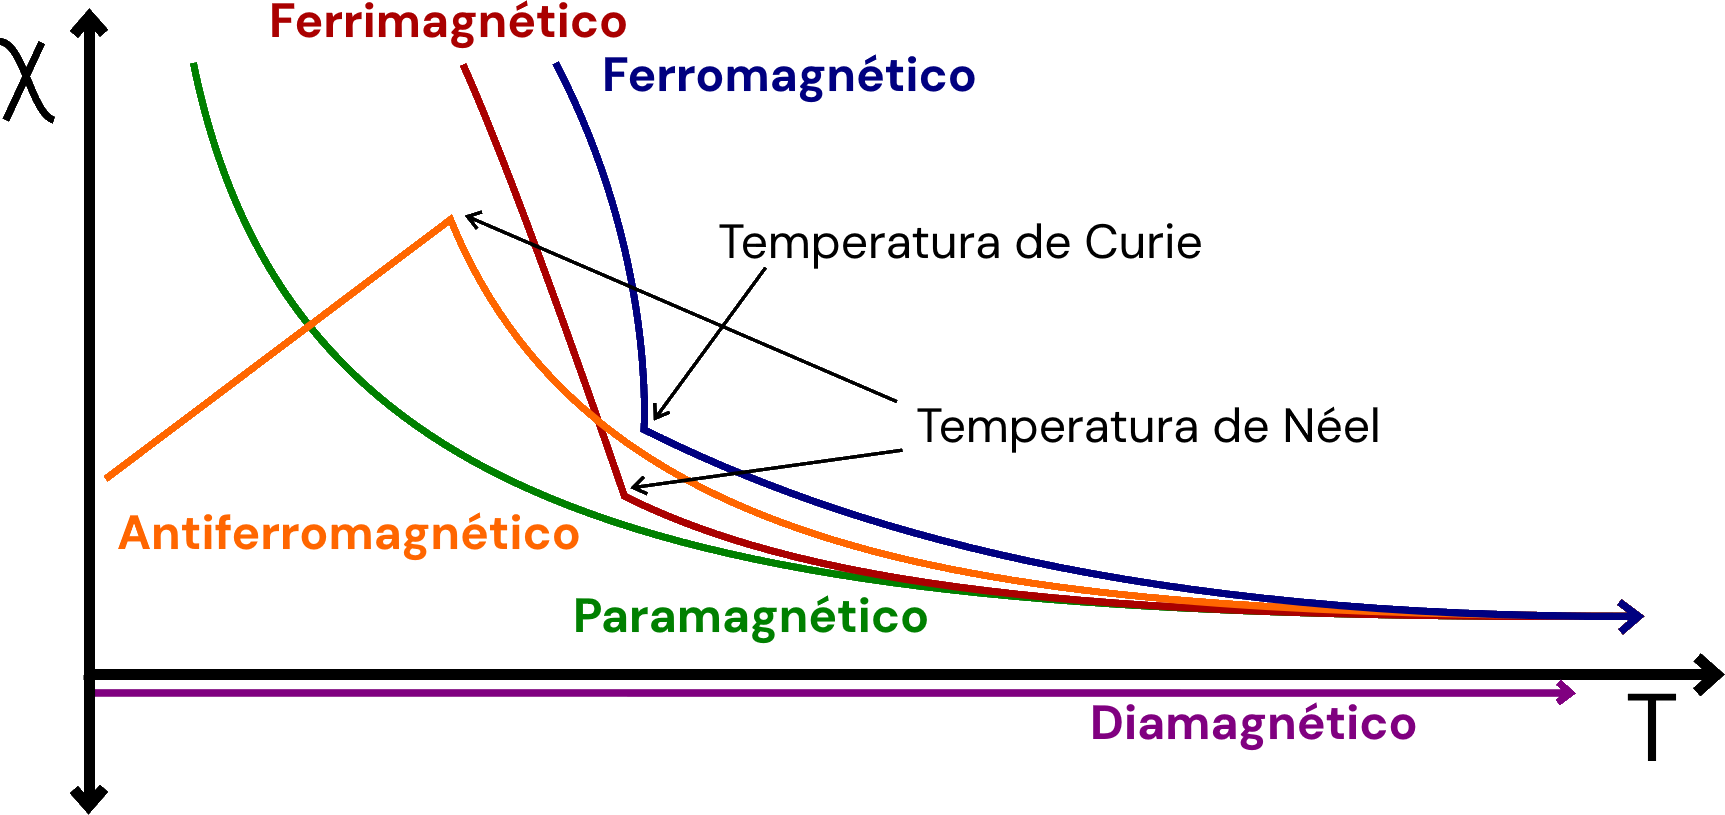
\includegraphics[width=0.75\textwidth]{fig/chitemp.png}
    \caption{Comportamiento de la susceptibilidad respecto a la temperatura para cada tipo de material. Adaptado de \cite{Ohl2021}.}
    \label{fig:chitemp}
\end{figure}
Los materiales magnéticos pueden clasificarse a través de su respuesta a los campos externos y a la temperatura a la que se encuentran. Es posible dividirlos en dos grupos:

\textbf{A. Materiales sin orden magnético intrínseco}
\begin{itemize}
    \item \textbf{Diamagnéticos:} Cuando los electrones son expuestos a un campo magnético externo ($H$), la torca que éste ejerce sobre el momento magnético del electrón ocasiona que éste rote periódicamente, lo cual a su vez genera un campo magnético en sentido opuesto al que fue aplicado debido a la Ley de Lens. La susceptibilidad se expresa como:
    \begin{equation}
        \chi_{\text{orb}}=\dfrac{-n_{\text{orb}}\mu_0e^2\avrg{r^2}}{6m_e}
        \label{eq:chidiamagorb}
    \end{equation}
    \begin{equation}
        \chi_L=\dfrac{-n_\text{libres}\mu_0\mu_B^2}{2k_BT_F}
        \label{eq:chidiamaglandau}
    \end{equation}
    Donde la contribución del diamagnetismo orbital $(\chi_\text{orb})$ toma en cuenta los electrones ligados ($n_\text{orb}$), y la del diamagnetismo de Landau $(\chi_L)$ los electrones libres ($n_\text{libres}$). Además, $n$ es el número de electrones del tipo correspondiente, $\mu_0$ la permeabilidad del vacío, $\mu_B$ el magnetón de Bohr, $k_B$ la constante de Boltzmann, $m_e$ y $e$ la masa y la carga del electrón respectivamente, $\avrg{r^2}$ el promedio del cuadrado de la posición de los electrones y $T_F$ la temperatura de Fermi. Ambas susceptibilidades son negativas y constantes en la temperatura \cite{coey2010magnetism}, como se observa en la línea morada de la figura \ref{fig:chitemp}, además, el comportamiento de sus espines se ilustra en la figura \ref{fig:magtiposdiag} a.
    \item \textbf{Paramagnéticos:} Cuando un material que posee electrones desapareados en su capa de valencia es expuesto a un campo magnético externo ($H$), se favorecerá el alineamiento de los momentos magnéticos de cada electrón en la dirección del campo. El campo ordena los momentos magnéticos, provocando una magnetización diferente de 0, la cual puede modelarse a través de las funciones de Brillouin y Langevin \cite{coey2010magnetism}.
    \begin{equation}
        B_J(x)=\dfrac{2J+1}{2J}\coth\left(\dfrac{2J+1}{2J}x\right)-\dfrac{1}{2J}\coth\left(\dfrac{x}{2J}\right)
        \label{eq:Brillouin}
    \end{equation}
    \begin{equation}
        L(x)=\coth(x)-\dfrac{1}{x}
        \label{eq:Langevin}
    \end{equation}
    Donde $J=L+S$ es la suma del momento angular y el espín total del átomo, y representa el momento angular total de los átomos que conforman el material. Cabe mencionar que $L(x)$ es el límite clásico de las funciones $B_J$ cuando $J\rightarrow\infty$, por lo que se puede utilizar cuando se tiene una gran cantidad de estados energéticos y se pueden aproximar como continuos. Por otro lado,
    \begin{equation}
        x=\dfrac{g\mu_B\mu_0M_JH}{k_BT}\qquad (B_J(x))
        \label{eq:xBrillouin}
    \end{equation}
    Donde $g$ es el factor de Landé y $M_J$ es el número cuántico magnético asociado al momento angular total.

    Para un campo $H$ en el eje $z$ se tiene que, en el caso del paramagnetismo:
    \begin{equation}
            \avrg{m_z}=g\mu_BJB_J(x) \implies M=ng\mu_B J B_J(x)
        \label{eq:momentozetaparam}
    \end{equation}
    \begin{equation}
        \implies \chi=\dfrac{ng\mu_B J B_J(x)}{H}=\dfrac{n g^2 \mu_B^2 J^2 \mu_0}{k_BT}\left(\dfrac{B_J(x)}{x}\right)
        \label{eq:chiparam}
    \end{equation}
    Cuando $x\ll1$, $B_J\approx(J+1)x/3J$, por lo que
    \begin{equation}
        \chi\approx\dfrac{ng^2\mu_B^2J(J+1)\mu_0}{3k_BT}=\dfrac{C}{T}
        \label{eq:leycurie}
    \end{equation}
    Esto se conoce como la ley de Curie, la cual da el comportamiento que se muestra en la curva verde de la figura \ref{fig:chitemp} y se ilustra en la figura \ref{fig:magtiposdiag} b. Cabe mencionar que este desarrollo es válido también utilizando la función $L(x)$ en lugar de $B_J(x)$ \cite{coey2010magnetism}.
\end{itemize}
\textbf{B. Materiales con orden magnético intrínseco}

Los materiales con orden magnético intrínseco poseen una magnetización interna, la cual se modela macroscópicamente con el campo medio de Weiss.

Este supone que el efecto de la magnetización al aplicar un campo $H$ da como resultado un campo neto $H^i$ de la forma:
\begin{equation}
    H^i=n_wM+H
    \label{eq:Weiss}
\end{equation}
Esto permite extender el análisis realizado para el paramagnetismo a través de funciones de Brillouin a los materiales con orden magnético intrínseco.

Este campo interno es generado principalmente por la interacción de intercambio, además de otras interacciones dentro del material. Para átomos en una red cristalina se degenera la energía de los electrones que existen en los orbitales enlazados, producto del principio de exclusión de Pauli.

Los electrones en este estado de energía, debido a que son indistinguibles entre sí, pueden ocupar cualquier orbital en la red correspondiente a electrones desapareados. Este comportamiento puede modelarse mediante el siguiente hamiltoniano:
\begin{equation}
    \mathcal{H}_\text{H}=-2\mathcal{J}\vec{S_i}\cdot\vec{S_j}
    \label{eq:hamiltonianoheisenberg}
\end{equation}
Donde $\mathcal{H}_\text{H}$ se conoce como el hamiltoniano de Heisenberg, $\vec{S_i}$ y $\vec{S_j}$ los espines totales de dos átomos vecinos y $\mathcal{J}$ es la integral de intercambio:
\begin{equation}
    \mathcal{J}=\int \psi^\ast_i(\vec{r}')\psi^\ast_j(\vec{r})\mathcal{H}(\vec{r},\vec{r}')\psi_i(\vec{r}')\psi_j(\vec{r})\text{d}^3r\text{d}^3r'
    \label{eq:intintercambio}
\end{equation}
Donde $\psi_k$ es la función de onda de probabilidad del átomo $k$-ésimo ($k=i,$ $j$).

El signo de esta integral determina qué orientación relativa de espines de átomos vecinos será favorecida por el cristal, si $\mathcal{J}>0$, será más energéticamente favorable que haya espines paralelos, mientras que con $\mathcal{J}<0$ lo mismo ocurrirá para espines antiparalelos, esto a su vez genera regiones del cristal con espines ordenados paralela o antiparalelamente, conocidas como dominios magnéticos \cite{coey2010magnetism}.

Cabe mencionar que, además de la interacción descrita por el hamiltoniano de Heisenberg, existe otra componente que describe la interacción entre átomos con espines perpendiculares, descrita por el hamiltoniano de Dzyaloshinskii-Moriya:
\begin{equation}
    \mathcal{H}_\text{DM}=-\vec{\mathcal{D}}\cdot\left(\vec{S_1}\times\vec{S_2}\right)
    \label{eq:hamiltonianoDM}
\end{equation}
Esta interacción tiende a alinear los espines de forma perpendicular, sin embargo, es de mucha menor magnitud al efecto del hamiltoniano de Heisenberg ($\mathcal{D}/\mathcal{J}\approx10^{-2}$), lo cual produce una desviación de alrededor de 1$^\circ$. Esto provoca que los materiales antiferromagnéticos presenten un momento ferromagnético pequeño \cite{coey2010magnetism} \cite{Dzyaloshinsky1958}.
\begin{itemize}
    \item \textbf{Ferromagnéticos $(\mathcal{J}>0)$ :} El signo de $\mathcal{J}$ provoca que los espines se alineen de forma paralela, lo cual produce que los dominios tengan una magnetización neta distinta de 0. Estos materiales presentan un cambio de fase en una temperatura determinada conocida como la temperatura de Curie, esto pues, al realizar el análisis hecho para el paramagnetismo con $H^i$ en lugar de $H$, se encuentra lo siguiente:
    \begin{equation}\begin{split}
        M=\dfrac{C}{T}H^i=\dfrac{C}{T}(n_wM+H)\\
        \implies M=\dfrac{C}{T-T_C}H\text{ , }n_wC=T_C\\
        \implies \chi=\dfrac{C}{T-T_C}
    \end{split}
        \label{eq:leycurieweiss}
    \end{equation}
    Donde $T_C$ se conoce como temperatura de Curie. Esta expresión se conoce como la ley de Curie-Weiss.

    Por debajo de la temperatura de Curie, los materiales ferromagnéticos presentan orden magnético intrínseco, cuando rebasan esta temperatura tienen un comportamiento paramagnético \cite{coey2010magnetism}, como se muestra en la curva azul de la figura \ref{fig:chitemp}, este comportamiento se ilustra en la figura \ref{fig:magtiposdiag} c.
    \item \textbf{Antiferromagnéticos ($\mathcal{J}<0$):} De manera similar a los materiales ferromagnéticos, existen dominios magnéticos producto de la interacción de intercambio en este tipo de material, sin embargo, los espines se alinean de manera antiparalela, puesto que $\mathcal{J}<0$. Esto genera dos subredes, cuyos espines apuntan en direcciones opuestas y son de igual magnitud. Al modelar estas dos subredes como campos medios independientes, se puede llegar a un análogo de la ley de Curie-Weiss:
    \begin{equation}
        \chi=\dfrac{C}{T+T_N}\qquad\text{Cuando }T>T_N
        \label{eq:tempdeneel}
    \end{equation}
    Donde $T_N$ es la temperatura de Néel. Esto representa un comportamiento paramagnético cuando $T>T_N$, cuando $T$ es menor, $\chi$ se vuelve menor debido al alineamiento antiparalelo de los espines, por lo que se tiene un máximo en $T=T_N$ \cite{coey2010magnetism}. Este comportamiento se muestra en la curva amarilla de la figura \ref{fig:chitemp}. El ordenamiento de los espines se ilustra en la figura \ref{fig:magtiposdiag} d.
    \item \textbf{Ferrimagnéticos ($\mathcal{J}<0$):} De manera similar a los materiales antiferromagnéticos, presentan dos subredes producto de la alineación antiparalela debido al signo de $\mathcal{J}$, tienen un comportamiento paramagnético sobre la temperatura de Néel, la cual se define como la que se muestra en la ecuación \ref{eq:tempdeneel}, sin embargo, las subredes no son de la misma magnitud, sino que una de ellas es mayor a la otra, provocando una magnetización neta distinta de 0 en los dominios cuando $T<T_N$, de forma similar a los materiales ferromagnéticos \cite{coey2010magnetism}. Este comportamiento se observa en la curva roja de la figura \ref{fig:chitemp}, mientras que la configuración de sus espines se ilustra en la figura \ref{fig:magtiposdiag} e.
    \item \textbf{Superparamagnéticos ($\mathcal{J}>0$):} Se trata de materiales ferromagnéticos compuestos de partículas cuyo tamaño es menor o igual que el de un dominio magnético, lo cual provoca que se comporten como una sola partícula paramagnética grande con un solo espín, conocido como \textit{macroespín}, lo cual se ilustra en la figura \ref{fig:magtiposdiag} f. La susceptibilidad de estas partículas sigue la ley de Curie, con un valor de $C$ muy grande, como se observa en la curva rosa de la figura \ref{fig:chitemp}. Sin embargo, a baja temperatura, la energía térmica no es suficiente para evitar el ordenamiento magnético entre partículas, por lo cual se comportan como ferromagnéticos a baja temperatura \cite{coey2010magnetism}.
\end{itemize}
\begin{figure}[H]
    \centering
    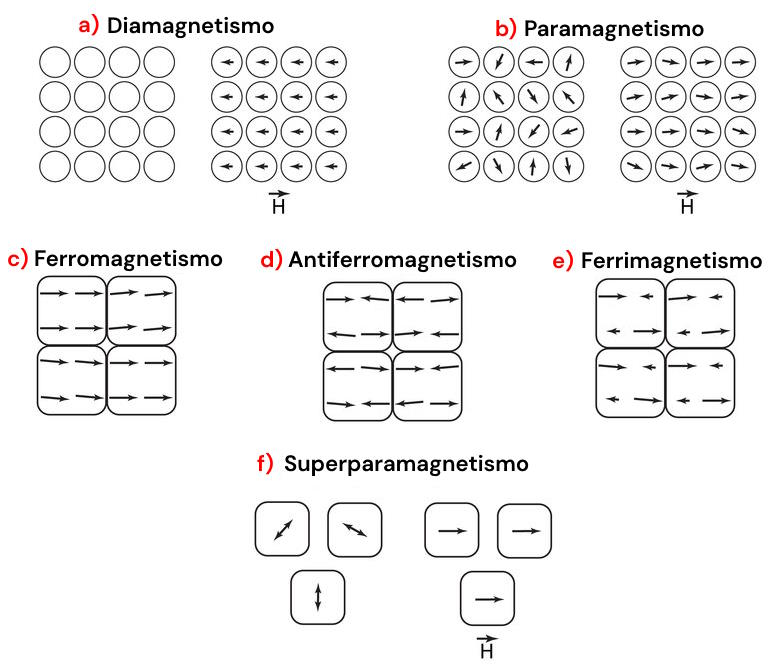
\includegraphics[width=0.7\textwidth]{fig/magtiposdiag.jpg}
    \caption{Diagrama de la configuración de los espines de cada tipo de material. Adaptado de \cite{Bloemen2015}.}
    \label{fig:magtiposdiag}
\end{figure}
\subsubsection{Curvas \texorpdfstring{$M$}{M} contra \texorpdfstring{$H$}{H}}
El comportamiento de la magnetización contra el campo externo depende del tipo de material. Esta dependencia puede explicarse con la ecuación \ref{eq:macromag}, donde se observa que la susceptibilidad define la relación entre ambos campos.
\begin{figure}[H]
    \centering
    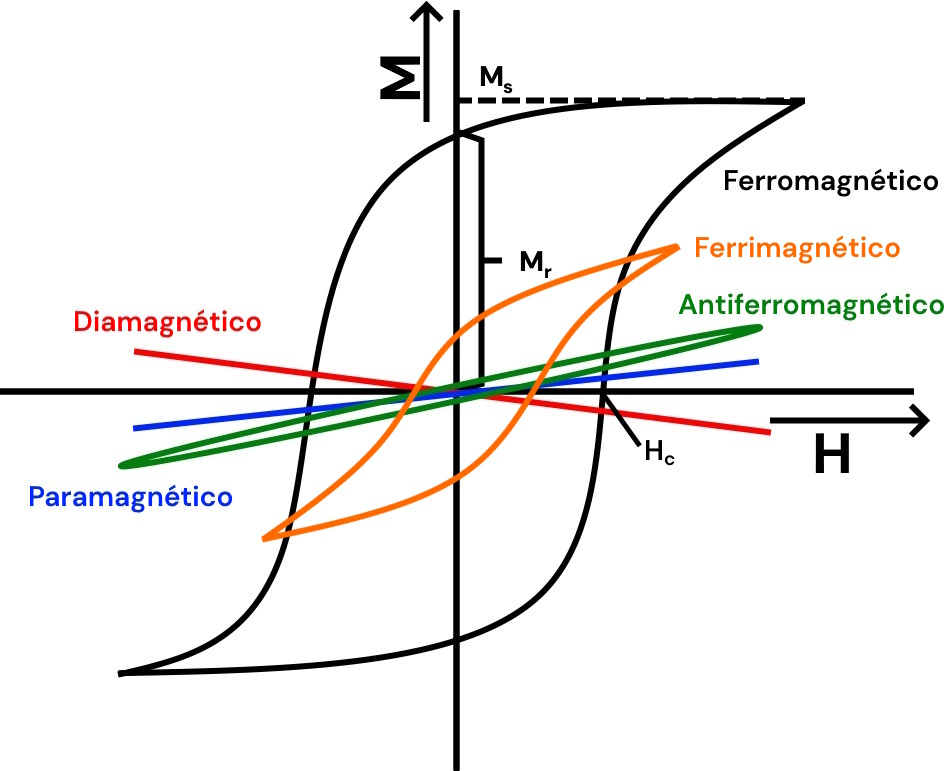
\includegraphics[width=0.55\textwidth]{fig/histeresis1.jpg}
    \caption{Comportamiento de la magnetización contra el campo para los distintos tipos de materiales magnéticos. Adaptado de \cite{Buschow2003}.}
    \label{fig:campomag}
\end{figure}
Los materiales sin orden magnético intrínseco tienen un comportamiento simple, el diamagnetismo tiene un comportamiento lineal con una pendiente negativa, como se ve en las ecuaciones \ref{eq:chidiamagorb} y \ref{eq:chidiamaglandau}, y el paramagnetismo puede aproximarse como lineal con una pendiente positiva en la región descrita para la ecuación \ref{eq:leycurie}. Ambos comportamientos pueden observarse en la figura \ref{fig:campomag}, la línea roja ilustra el comportamiento de un diamagneto, y la azul la de un paramagneto.

Por otro lado, los materiales con orden magnético intrínseco presentan histéresis, es decir, su estado actual no depende sólo de las condiciones en las que se encuentran, sino también de las condiciones pasadas del sistema.

Esto tiene su origen en las interacciones magnéticas en el cristal, en particular la de intercambio y la anisotropía, éstas hacen energéticamente más favorable que los espines estén alineados en dominios magnéticos, lo cual provoca que, al aplicar un campo externo $H$, los dominios cuya magnetización es paralela al campo aplicado comienzan a crecer a costa de aquellos con otra orientación.

Para estos materiales podemos definir:
\begin{itemize}
    \item \textbf{Magnetización de saturación ($M_s$):} Esta se refiere al valor constante que toma la magnetización cuando todos los espines se han alineado con el campo externo, impidiendo que esta crezca más.
    \item \textbf{Magnetización remanente ($M_r$):} Cuando un material con orden magnético intrínseco es expuesto a un campo externo y posteriormente este es retirado, la magnetización no regresa a 0, sino que el material mantiene una magnetización remanente.
    \item \textbf{Campo coercitivo ($H_c$):} Se refiere al campo necesario para que la magnetización de un material con orden magnético intrínseco regrese a 0 después de haberle aplicado un campo externo.
\end{itemize}
Aunque todos los materiales con momento magnético intrínseco, excepto los superparamagnéticos, exhiben histéresis, las características de ésta varían significativamente entre diferentes tipos de materiales, como se ilustra en la Figura \ref{fig:campomag}. Los materiales ferromagnéticos (representados por la curva negra) presentan los valores más altos de $M_r$, $M_s$ y $H_c$, superando notablemente a los observados en sistemas ferrimagnéticos (curva naranja) y antiferromagnéticos (curva verde). Este último grupo muestra un comportamiento distinto, los materiales antiferromagnéticos se caracterizan por ciclos estrechos con apariencia elíptica, mientras que los ferrimagnéticos presentan curvas intermedias entre ambos comportamientos.

En el caso de los superparamagnéticos $H_c,M_r=0$, es decir, su magnetización regresa al estado inicial en ausencia de un campo externo, de la misma forma en la que lo haría un paramagnético, este comportamiento se observa en la curva rosa de la figura \ref{fig:campomag}.
\subsection{Polarización en Sólidos}
Podemos distinguir dos categorías de sólidos, conductores, donde las cargas eléctricas pueden desplazarse libremente, y dieléctricos, donde existen cargas ligadas. Son éstas últimas las que dan lugar a la polarización, por lo cual, esta sólo existe en dieléctricos.

En sólidos cristalinos dieléctricos anisótropos, podemos expresar las componentes vectoriales de la primer ecuación \ref{eq:maxwellmacro} como:
\begin{equation}
    D_i=P_{0i}+\varepsilon_{ik}E_k
    \label{eq:macroelec}
\end{equation}
Con $\vec{P_{0}}$ la polarización espontánea del cristal y $\varepsilon_{ik}$ un tensor de rango 2 que representa la permitividad eléctrica según la dirección.

Por simetría, esta polarización debe ser invariante ante las mismas transformaciones que la celda unitaria, esto sólo es posible para una polarización espontánea diferente de 0 si la dirección $\hat{P_{0}}$ permanece constante ante estas transformaciones lo cual se conoce como simetría polar.

Si el sólido es centrosimétrico, es decir, tiene un punto de simetría, $P_0=0$, se considera un paraeléctrico, su polarización está dada completamente por el campo externo, es decir, tienen una respuesta lineal, análoga a los materiales paramagnéticos.


De manera análoga al magnetismo, es posible definir la polarización del material $\vec{P}$ como:

\begin{equation}
    \vec{P}=\dfrac{1}{V}\sum_{i}\vec{P_{0i}}
    \label{eq:polarizacionmicromacro}
\end{equation}
Donde $\vec{P_{0i}}$ es la polarización espontánea de la celda cristalina $i$-ésima.

La polarización espontánea de un sólido deforma a las cargas ligadas de la misma forma en la que lo haría el aplicar un campo externo, dando lugar a carga en la superficie del sólido, lo cual provoca un campo de depolarización $\vec{E_\text{dep}}$ en el sentido opuesto a $\vec{P_0}$. Estas cargas ligadas provocan el movimiento de cargas libres en el sistema, por lo cual, al llegar al equilibrio, el campo externo es 0, esto se ilustra en la figura \ref{fig:ferroelecdiag}.
\begin{figure}[H]
    \centering
    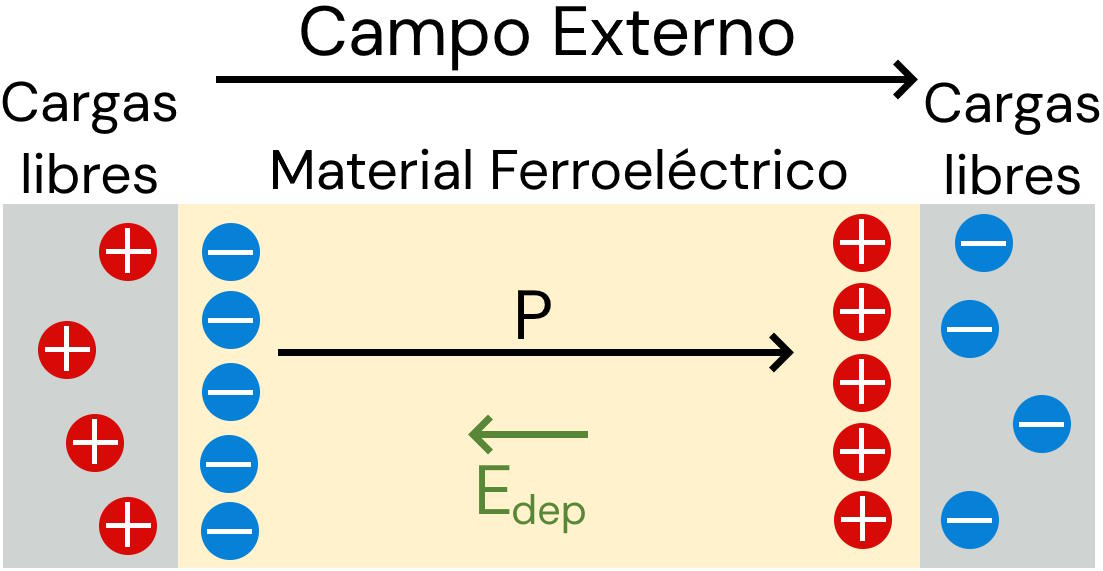
\includegraphics[width=0.7\textwidth]{fig/ferroelecdiag.jpg}
    \caption{Diagrama de la configuración de cargas en un ferroeléctrico. Adaptado de \cite{Qiao2021}.}
    \label{fig:ferroelecdiag}
\end{figure}
Sin embargo, al variar la temperatura, las posiciones de los átomos en la celda cristalina cambian ligeramente, lo cual provoca un movimiento de las cargas superficiales, generando una corriente, este fenómeno se conoce como piroelectricidad.

Las modificaciones a una red cristalina pueden incluir fases piroeléctricas y fases paraeléctricas, si el cambio de una a otra se da a través de una transición de segundo orden, cerca del punto de transición, conocido como punto de Curie, se tienen propiedades distintas de las esperadas de un piroeléctrico.

En un cristal piroeléctrico, el cambio de dirección de la polarización espontánea requiere de un cambio muy grande en la estructura cristalina, lo cual requiere de una gran cantidad de energía, incluso si el resultado fuese energéticamente favorable.

Cerca de el punto Curie, la energía necesaria para cambiar la dirección de polarización no es tan grande debido a que $\vec{P_{0}}$ es más pequeño, además de que la estructura cristalina está cerca de una configuración paraeléctrica, lo cual produce un comportamiento conocido como ferroelectricidad.

El hecho de que esta deformación sea posible hace que $E_\text{dep}$ pueda cambiar la dirección de polarización espontánea de las celdas cristalinas.

La energía $U_\text{dep}$ proveniente del campo de depolarización se puede escribir como:
\begin{equation}
    U_\text{dep}=\dfrac{1}{2}\varepsilon_0\varepsilon_r\int|E_\text{dep}|^2dV\propto\dfrac{P^2}{2\varepsilon_0\varepsilon_r}V
    \label{eq:energiadepolarizacion}
\end{equation}
Con $\varepsilon_r$ la permitividad relativa del material.

Se observa que esta depende del volumen, es decir, se ve minimizada con este, lo cual favorece energéticamente la aparición de dominios de polarización.

La energía libre $F$ de un ferroeléctrico se expresa de la siguiente manera:
\begin{equation}
    F=\underbrace{\alpha(T-T_c)P^2+\beta P^4}_\text{\clap{Potencial de Landau}}+\underbrace{\dfrac{1}{2\varepsilon_0\varepsilon}P^2}_\text{\clap{Depolarización}}+\dots
    \label{eq:energíalibre}
\end{equation}
Donde $\alpha$ y $\beta$ son coeficientes que describen el comportamiento del sistema cerca de la temperatura de Curie.

$F$ tiene un mínimo en $P=\pm P_{0}$, además, es estable en $P=0$ (fase paraeléctrica) $P=\pm P_{0}$ (fase ferroeléctrica) \cite{Landau1984}.
\subsubsection{Curvas \texorpdfstring{$P$}{P} contra \texorpdfstring{$E$}{E}} \label{sec:PEarte}
Al realizar mediciones de polarización contra campo, es importante considerar la corriente suministrada para generar el campo, debido a que la carga ($Q$) puede expresarse como:
\begin{equation}
    Q=\int_{t_1}^{t_2}I(t)\text{d}t
    \label{eq:cargaintensidad}
\end{equation}
Donde $I$ es la corriente que se hace pasar a través de la muestra en el tiempo $t$.
Con esto, podemos expresar el desplazamiento dieléctrico ($D$) como:
\begin{equation}
    D(t)=\dfrac{Q}{A}
    \label{eq:despdielec}
\end{equation}
Donde $A$ es el área superficial de la muestra.
\begin{equation}
    P(t)=D(t)-\epsilon_0E(t)
    \label{eq:polarizacionec}
\end{equation}
A través de estas mediciones es posible determinar el tipo de material que se tiene \cite{Stewart1999}.
\begin{figure}[H]
    \centering
    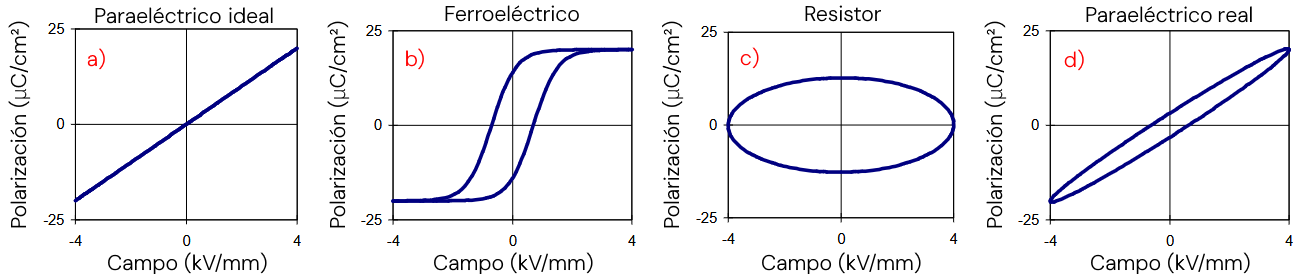
\includegraphics[width=0.9\textwidth]{fig/PEloop.png}
    \caption{Curvas de Polarización para distintos tipos de Material. Adaptado de \cite{Stewart1999}.}
    \label{fig:PEloop}
\end{figure}
\begin{itemize}
  \item \textbf{Paraeléctricos:} Tienen una relación lineal entre $P$ y $E$, independiente de la forma de $I(t)$, como se observa en la figura \ref{fig:PEloop} a.
  \item \textbf{Ferroeléctricos:} Presentan histéresis, dando como resultado curvas de polarización como la que se observa en la figura \ref{fig:PEloop} b.
  \item \textbf{Resistores:} No tienen una relación entre $P$ y $E$ independiente de la corriente aplicada, sino que su comportamiento depende de ésta. Dada la integral con la que se obtiene $Q$, si se aplica un campo senoidal, la polarización será cosenoidal, dando como resultado una curva como la que se observa en la figura \ref{fig:PEloop} c.
\end{itemize}
Finalmente, es necesario mencionar que la polarización de los paraeléctricos reales pueden tener cierta dependencia con la corriente, dando lugar a un comportamiento intermedio en la curva de polarización, como se observa en la figura \ref{fig:PEloop}d.
\subsubsection{Multiferroicidad} \label{sec:multif}
Los materiales multiferróicos son aquellos que presentan orden intrínseco en más de una de sus propiedades. En particular son relevantes para este trabajo aquellos que presentan orden magnético y orden eléctrico.

En estos materiales existe un efecto de acoplamiento entre las respuestas magnética y eléctrica, dando como resultado que el aplicar un campo magnético produzca cambios en la polarización, y el aplicar un campo eléctrico produzca cambios en la magnetización.

La fuerza de este acoplamiento puede describirse mediante las siguientes constantes:
\begin{equation}
    \alpha_E=\left(\dfrac{\partial M}{\partial E}\right)
    \label{eq:alphaE}
\end{equation}
\begin{equation}
    \alpha_H=\left(\dfrac{\partial P}{\partial H}\right)=\varepsilon_0\varepsilon_r\left(\dfrac{\partial E}{\partial H}\right)
    \label{eq:alphaH}
\end{equation}
Donde $\varepsilon_r$ es la permitividad relativa del sólido. Asumiendo una muestra cilíndrica delgada de grosor $t$, el voltaje puede escribirse como $V=E/t$, por lo que:
\begin{equation}
    \alpha_H=\dfrac{\varepsilon_0\varepsilon_r}{t}\left(\dfrac{\partial V}{\partial H}\right)=\varepsilon_0\varepsilon_r\alpha_H^V
    \label{eq:alphaHV}
\end{equation}
Donde $\alpha_H^V$ se conoce como coeficiente  magneto-eléctrico de voltaje inducido magnéticamente.

Este acoplamiento es lo que hace a estos materiales de interés particular, ya que permite un gran número de aplicaciones, como detectores de campo magnético de alta precisión (campos del orden de $\sim10^{-12}$ T) a temperatura ambiente, aparatos de resonancia ferromagnética (FMR) sintonizables eléctricamente, además de aplicaciones en el manejo y procesamiento de señales, además de el almacenamiento de datos, entre otras \cite{Vopson2015}.
\subsection{Propiedades de las ortoferritas de tierras raras}
\subsubsection{Propiedades magnéticas}
Las ortoferritas \ce{RFeO3} presentan un comportamiento antiferromagnético (AFM) a temperatura ambiente, con un ferromagnetismo débil inducido por la interacción de Dzyaloshinskii-Moriya.

Se pueden distinguir tres tipos de orden antiferromagnético en las ortoferritas de tierras raras \cite{KamalWarshi2018}:
\begin{figure}[H]
    \centering
    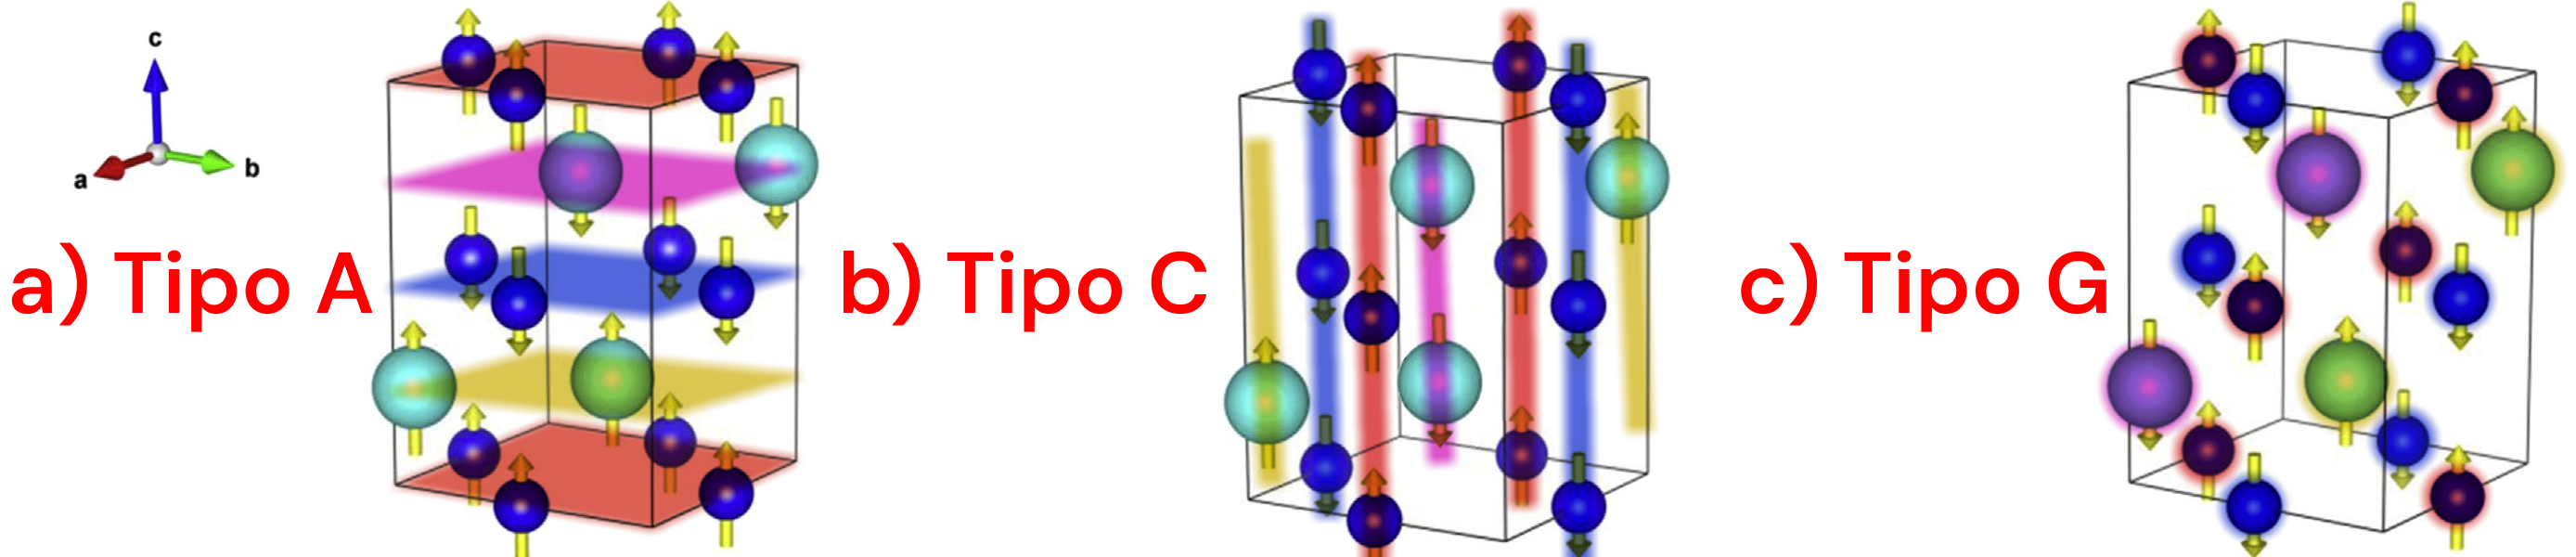
\includegraphics[width=0.8\textwidth]{fig/tiposAFM.png}
    \caption{Tipos de orden antiferromagnético en las ortoferritas \ce{RFeO3}. Adaptado de \cite{Wang2019}. Observe que existen dos pares de subredes superpuestas, un par compuesto por los átomos de R (marcados en amarillo y rosa), y otro compuesto por los átomos de Fe (marcados en rojo y azul).}
    \label{fig:tiposAFM}
\end{figure}
\begin{itemize}
    \item \textbf{AFM tipo A:} (figura \ref{fig:tiposAFM} a) los espines se alinean en planos paralelos al plano $ab$ dentro de una misma capa pero alternan su orientación entre capas adyacentes.
    \item \textbf{AFM tipo C:} (figura \ref{fig:tiposAFM} b) los espines se alinean a lo largo de una línea paralela al eje $c$, alternando su orientación entre líneas paralelas.
    \item \textbf{AFM tipo G:} (figura \ref{fig:tiposAFM} c) los espines alternan su orientación respecto a sus primeros vecinos.
\end{itemize}
Esto tiene como consecuencia que estos materiales presenten transiciones de fase magnéticas al variar la temperatura, producto de un reacomodo de sus espines.

\subsubsection{Propiedades eléctricas}
\begin{figure}[H]
    \centering
    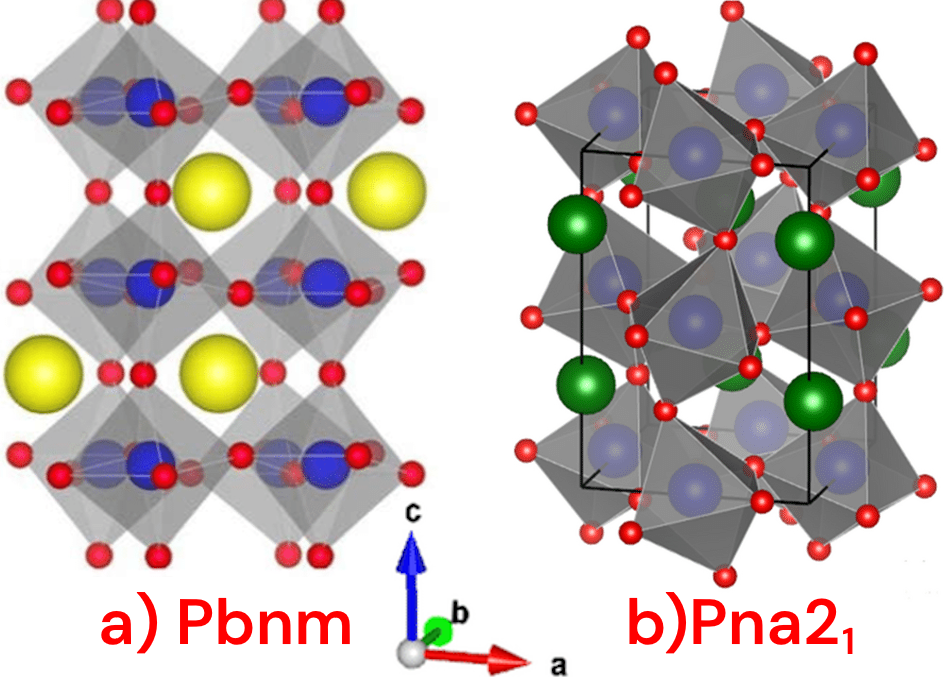
\includegraphics[width=0.6\textwidth]{fig/estructurascristalinas.png}
    \caption{Posibles estructuras cristalinas de las ortoferritas estudiadas. Adaptado de \cite{Herklotz2021} y \cite{Oumertem2019}.}
    \label{fig:estructcrist}
\end{figure}
Aunque la simetría de la estructura cristalina $Pbnm$ (figura \ref{fig:estructcrist} a) no permite la ferroelectricidad, se ha observado que el calentamiento de estas ferritas induce una transición de fase hacia una estructura $Pna2_1$ (figura \ref{fig:estructcrist} b), la cual corresponde a una celda primitiva con un plano de reflexión perpendicular al eje $a$, un plano de deslizamiento perpendicular a $b$ y un eje helicoidal a lo largo de $c$, las cuales son simetrías compatibles con la ferroelectricidad \cite{Zhang2016}, \cite{Rajaitha2022}.

La coexistencia de orden magnético y eléctrico en estas fases las posiciona como candidatas ideales para aplicaciones multiferroicas, como las que se detallan en la sección \ref{sec:multif}.
\chapter{Objetivo}
\textbf{Objetivo general:}

Determinar cómo la temperatura de calcinación en la síntesis sol-gel de las ortoferritas \neod{} y \sama{} influye en sus propiedades magnéticas, eléctricas, ópticas, morfológicas y estructurales, así como evaluar la presencia de multiferroicidad en estos materiales.

\textbf{Objetivos específicos:}
\begin{itemize}
    \item Relacionar las condiciones de síntesis (temperatura de calcinación y tiempo de sonicación) con las propiedades estructurales, morfológicas, ópticas, magnéticas y eléctricas de las ortoferritas.
    \item Caracterizar las propiedades magnéticas (curvas $M$ vs. $H$, transiciones de espín a bajas temperaturas) y eléctricas (histéresis $P$ vs. $E$), para identificar correlaciones con la temperatura de síntesis y la posible coexistencia de orden en ambos parámetros.
    \item Determinar si las muestras presentan multiferroicidad, analizando la simultaneidad de ordenamiento ferroeléctrico y magnético, así como su sensibilidad a las condiciones de síntesis.
\end{itemize}
\textbf{Preguntas centrales de investigación:}

¿Cómo varían las propiedades magnéticas, eléctricas, ópticas y estructurales de \neod{} y \sama{} en función de la temperatura de calcinación durante su síntesis por sol-gel y su tiempo de sonicación? ¿Presentan estos materiales multiferroicidad?
\end{document}